\section{Correction with entanglement}

\begin{figure}[ht!]
	\centering
	\begin{subfigure}[t]{0.49\linewidth}
		\centering
		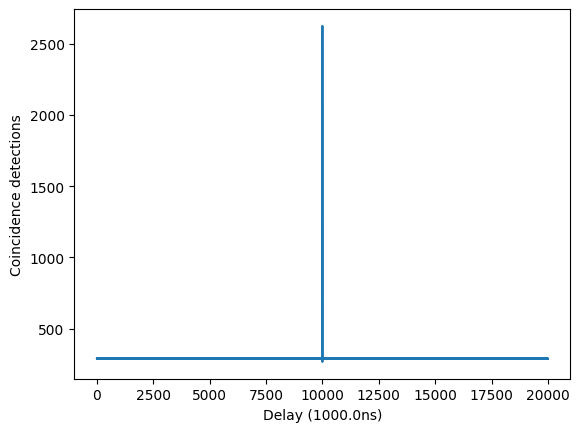
\includegraphics[height=4cm]{assets/unshifted_cc.png}
		\subcaption{}
	\end{subfigure}
	\begin{subfigure}[t]{0.49\textwidth}
		\centering
		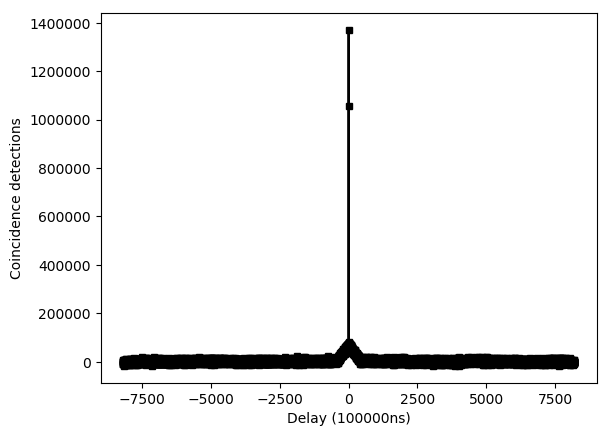
\includegraphics[height=4cm]{assets/firstDoppler_cc.png}
		\subcaption{}
	\end{subfigure}
	\caption{Autocorrelation of signal with (a) no shift (b) propagation delay}
	\label{fig:firstDoppler_cc}
\end{figure}
\begin{figure}[ht!]
	\centering
	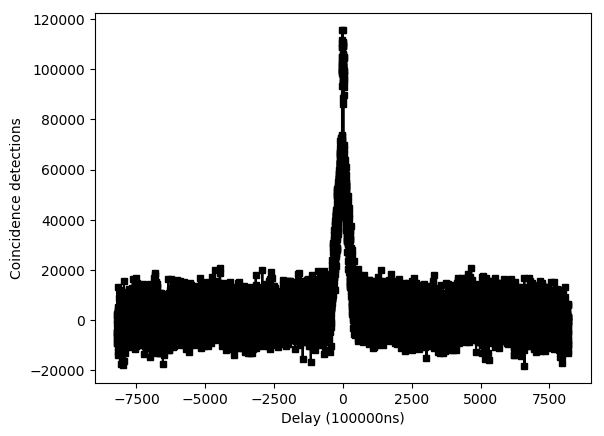
\includegraphics[width=0.95\linewidth]{assets/secondDoppler_cc.png}
	\caption{Autocorrelation of signal with delay and Doppler shift}
	\label{fig:secondDoppler_cc}
\end{figure}

\subsection{Ambiguity function}
The two-dimensional ambiguity function is commonly used in radar signal  analysis as the most complete statement of the waveform's inherent performance. It reveals the range-Doppler position of ambiguous re-sponses and defines the range and Doppler resolution. It is defined as 

\begin{equation}
A(\nu,\tau)\equiv\int_{-\infty}^{\infty}\tilde{s}\big(t+\frac{\tau}{2}\big)\tilde{s}^*\big(t-\frac{\tau}{2}\big)e^{2i\pi\nu t} dt
\end{equation}

\texttt{TODO: fill in machine learning method}

\begin{enumerate}
	\item find middle part with no shift
	\item try to shift middle part and find differential equation (order 2)
\end{enumerate}
 